% CHAPITRE 4
\singlespacing
\chapter{Effets de l'hydrologie sur les flux de GES}
\label{ch:4}

\minitoc

\newpage
\doublespacing
%\section{Manipulation du niveau de l'eau en mésocosmes}
\section{Introduction}

Au cours des deux années de suivis des flux de \coo et de \chh sur la tourbière de La Guette, le niveau de la nappe a très faiblement varié comparé aux années précédentes bien plus sèches.
En conséquence l'effet des variations de nappe sur les flux n'a pu être investigué.
% de cette faible variation peu de variations des flux ont pu y être relié.
Néanmoins l'hydrologie est un facteur contrôlant des flux \plop.
Ainsi de nombreuses études ont reliées les émissions de \coo au niveau de la nappe \plop.
Cependant, aucun consensus n'a encore été atteint :
La majorité des études montrent qu'une tourbière dont le niveau de la nappe est abaissé, soit par un drainage, soit par une sécheresse, aura tendance à avoir un ENE plus faible.
Par exemple, \citet{strack2013} expliquent des valeurs d'ENE plus faibles qu'escompté, par des mesures faites pendant une période relativement sèche.
Une observation similaire est faite par \citet{aurela2007} qui mesure un ENE plus faible lors d'une année sèche, sur une tourbière à Carex du sud de la Finlande.
Ils attribuent la variation de l'ENE à une augmentation de la RE et à une baisse de la PPB, dans des conditions plus chaudes et plus sèches.
\citet{peichl2014} observent également une baisse de l'ENE lors d'une année ou le niveau de la nappe baisse de façon importante, au delà de \SI{-30}{\centi\metre}.
Ils expliquent cette baisse par une baisse de la PPB.
Cette observation va dans le même sens que \citet{lund2012} qui observent en 2008 une baisse de l'ENE sur une tourbière à sphaignes située au sud de la suède.
% dont la végétation, Calluna vulgaris, Erica tetralix, Eriophorum vaginatum
Les mesures de RE faites cette année là étant similaires à celles effectuées les autres années, ils lient cette baisse à une diminution de la PPB.
En 2006, sur la même tourbière, \citet{lund2012} observent une autre baisse de l'ENE.
Mais cette fois, les mesures de PPB à leur tour similaires à celle des autres années n'expliquent pas cette baisse.
À l'inverse de 2008, cette baisse est expliqué par une augmentation de la RE.
Ces inconsistances apparentes peuvent avoir pour origine des types de sécheresse différente : courte et intense pendant la saison de végétation de 2006 et d'intensité plus faible mais d'une durée plus longue en 2008.
À l'inverse des résultats précédemment cités, \citet{ballantyne2014} dans une étude des effets à long terme d'une baisse du niveau de la nappe, observent pas d'effets significatifs sur l'ENE tandis que les flux de RE et de PPB augmentent tous les deux.
Ces études montrent que si le niveau de la nappe est reconnu comme un facteur de contrôle des flux de \coo, il est difficile d'en dégager des liens de cause à effet répétables.

Concernant le méthane, une baisse du niveau de la nappe est généralement liée à une baisse des émissions de \chh, et inversement, le niveau de la nappe contrôlant la proportion des zones ou le \chh est produit/oxydé \citep{pelletier2007}.
\citet{turetsky2008} montrent par ailleurs que selon leur sens, l'effet des variations du niveau de nappe sur les flux de \chh n'est pas identique.
Ils observent ainsi que l'effet est plus important lorsque le niveau de la nappe est augmenté que lorsqu'il est diminué ($\pm$ \SI{10}{\centi\metre}).
Ils font l'hypothèse que le niveau de la nappe, en plus de jouer sur la proportion production/oxydation, a un effet sur le transfert de chaleur dans le sol.
Cette hypothèse s'appuie sur l'observation de températures plus élevées, que ce soit celles de l'air ou de la tourbe, dans les zones ou le niveau de la nappe a été rehaussé.
Cependant d'autres études, principalement dans des sites ou le niveau de la nappe est proche de la surface du sol, montrent une absence de relation entre le niveau de la nappe et les émissions de méthane, voire une relation inverse, avec des flux plus faibles liés à des niveaux de nappe plus élevés \citep{kettunen1996,bellisario1999,treat2007}.
Là encore selon les conditions environnementales, la relation entre les flux de \chh et le niveau de la nappe n'est pas aisément généralisable.

La vitesse de l'augmentation du niveau de nappe semble également jouer sur les flux, des pics de RE ont été observés après la réhumectation rapide 
La façon dont le niveau de la nappe augmente semble également jouer sur les flux.
\citet{strack2009} ont observés qu'une hausse graduelle par le bas de la colonne de sol conduit à une baisse de la RE, tandis qu'une hausse rapide simulant un événement pluvieux (par le haut) conduisait à un pic de RE.
Ce pic de RE après une réhumectation a également été observé par \citet{mcneil2003}.
L'objectif de ce chapitre est donc d'explorer plus en avant l'effet du niveau de la nappe d'eau sur les émissions de GES, effet peu ou pas visible \textit{in-situ}.
Plus précisément il s'agit de déterminer l'effet de cycles de dessication/ré-humectation sur les émissions de \coo et de \chh. 
On attend donc qu'une baisse du niveau de la nappe une augmentation des flux de RE, avec possiblement un pic d'émission au moment de la réhumectation, et une diminution des flux de méthane.
(\plop cycle multiples effet)
%\citet{treat2007} montre également que selon l'échelle de temps le niveau de la nappe peut être corrélé soit négativement, soit positivement avec les flux de \chh.

\section{Procédure expérimentale}

L'étude des cycles de dessication/ré-humectation est effectuée sur des mésocosmes, prélevés à la tourbière de La Guette.
L'expérimentation a été réalisée durant l'été 2013 avec un seul cycle relativement long, on s'y référera par la suite comme l'expérimentation A.
L'expérimentation a été renouvelée l'été 2014 avec trois cycles, plus courts.
On appellera cette seconde expérimentation, l'expérimentation B (Tableau~\ref{table:recap_hm}).

\subsection{Expérimentation A}
Six mésocosmes ont été prélevés le 12 avril 2013, sur la tourbière de La Guette.
Le prélèvement s'effectue à l'aide de cylindres de PVC qui, dans un premier temps, posé sur le sol, permettent de faire un pré-découpage au couteau, puis dans un second temps sont insérés, délicatement, dans la tourbe. 
Les mésocosmes sont finalement dégagés en creusant de chaque côté (Figure~\ref{fig:mesophoto}).
Les mésocosmes sont transportés au laboratoire ou ils sont enterrés en extérieur et saturé en eau (eau prélevée dans la tourbière), afin que leur conditions hydrologique de départ soient les plus proche possible (Figure~\ref{fig:mesocarte}).
Trois mésocosmes tirés au sort servent de contrôle, et trois vont subir un cycle de dessication/ré-humectation.
%À partir du 31 mars 2013 de l'eau a été pompé régulièrement dans les 3 mésocosmes traités pour simuler une sécheresse, jusqu'au 17 juillet.
À partir du 31 mars 2013 les précipitations ont été interceptées à l'aide d'abri bâchés installable en cas de pluie et la nuit.
Ces interceptions ont été faites jusqu'au 17 juillet dans les 3 mésocosmes traités pour simuler une sécheresse.
À cette date de l'eau est ajouté aux mésocosmes, que ce soit les contrôles ou les traitements, pour simuler de fortes précipitations.

\subsection{Expérimentation B}
Le 17 avril 2014, six nouveaux mésocosmes ont été prélevés sur la tourbières de La Guette et installés près du laboratoire, en suivant le même protocole que pour l'expérimentation A.
Une station météo a été installée à côté des mésocosmes afin de mesurer la température de l'air, l'humidité relative, le rayonnement solaire, la vitesse et la direction du vent et les précipitations toutes les 15 minutes.
Cette station permettait également l'enregistrement des températures mesurées par des sondes (T107) installées à \num{-5}, \num{-10}, et \SI{-20}{\centi\metre}.
Les conditions météorologiques moins ensoleillée qu'en 2013 et l'objectif de suivre plusieurs cycles de dessiccation/réhumectation ont nécessité la mise en place d'un abaissement manuel du niveau de la nappe.
Pendant les phases d'assèchement les niveaux de nappes des placettes traitées étaient donc abaissés en moyenne de \SI{2.5}{\centi\metre} par jour.
Le premier cycle de dessication/réhumectation dura du 30 juin au 6 juillet pour la phase de dessication est du 7 au 16 juillet pour la phase de réhumectation.
Le deuxième cycle dura du 17 au 28 juillet et du 29 juillet au 3 aout, 
Enfin le dernier cycle fut mesuré du 4 au 11 aout pour la dessication et du 12 au 14 aout pour la réhumectation.

\subsection{traitement}

Pour les deux expérimentations les variables explicatives sont la température de l'air, du sol à \SI{-5}{\centi\metre}, le niveau de nappe, et l'humidité du sol. La végétation n'a été suivie que lors de l'expérimentation B.
Les placettes subissant les cycles de dessiccation seront nommées groupe « Dessiccation » et les placettes ne subissant pas les cycles, groupe « Contrôle ».
Ces deux groupes correspondent aux deux traitements utilisés pour l'analyse statistique.
Pour le \coo, l'analyse a été faite sur les flux moyennés sur une journée, les flux ayant été généralement mesuré deux fois par jour.
Pour le \chh, les flux bruts ont été utilisés.

\begin{figure}
\centering

\includegraphics[width=\textwidth]{chap4/mesocosmes}\\
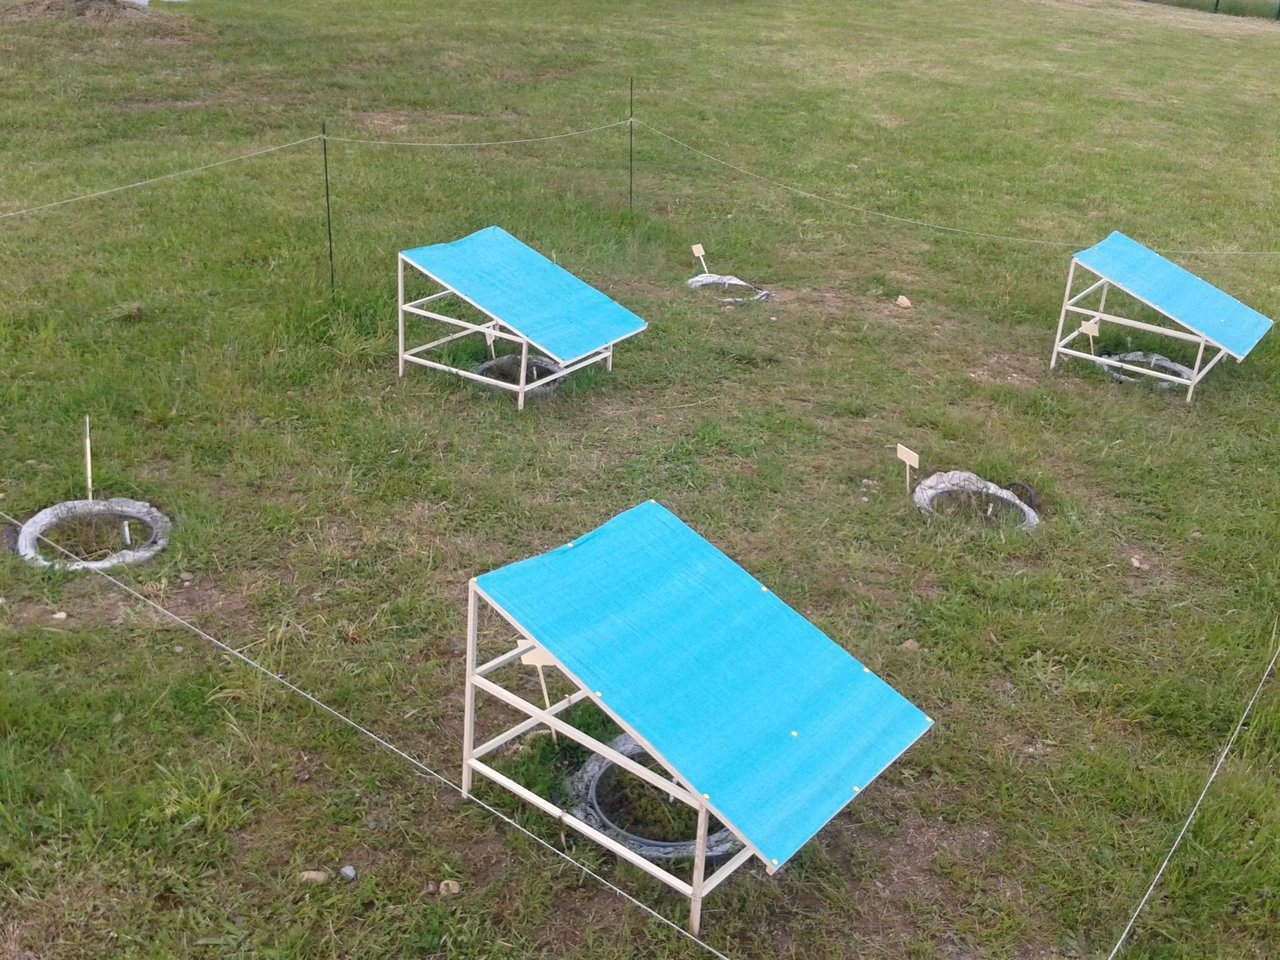
\includegraphics[width=\textwidth]{chap4/zi_exp_low}
\caption{Prélèvement des mésocosmes (en haut). Mésocosmes installés et protégés de la pluie (en bas).}
\label{fig:mesophoto}
\end{figure}


%\begin{table}
%\centering
%\caption{Récapitulatif des mesures pour les deux expérimentations}
%\label{table:recap_hm}
%\begin{tabular}{lll}\toprule
%expérimentation & A & B \\ \midrule
%année & 2013 & 2014 \\
%réplicats & 6 & 6 \\
%cycles & 1 & 3 \\
%station météo & non & oui\\
%\bottomrule
%\end{tabular}
%\end{table}


\begin{figure}
\centering
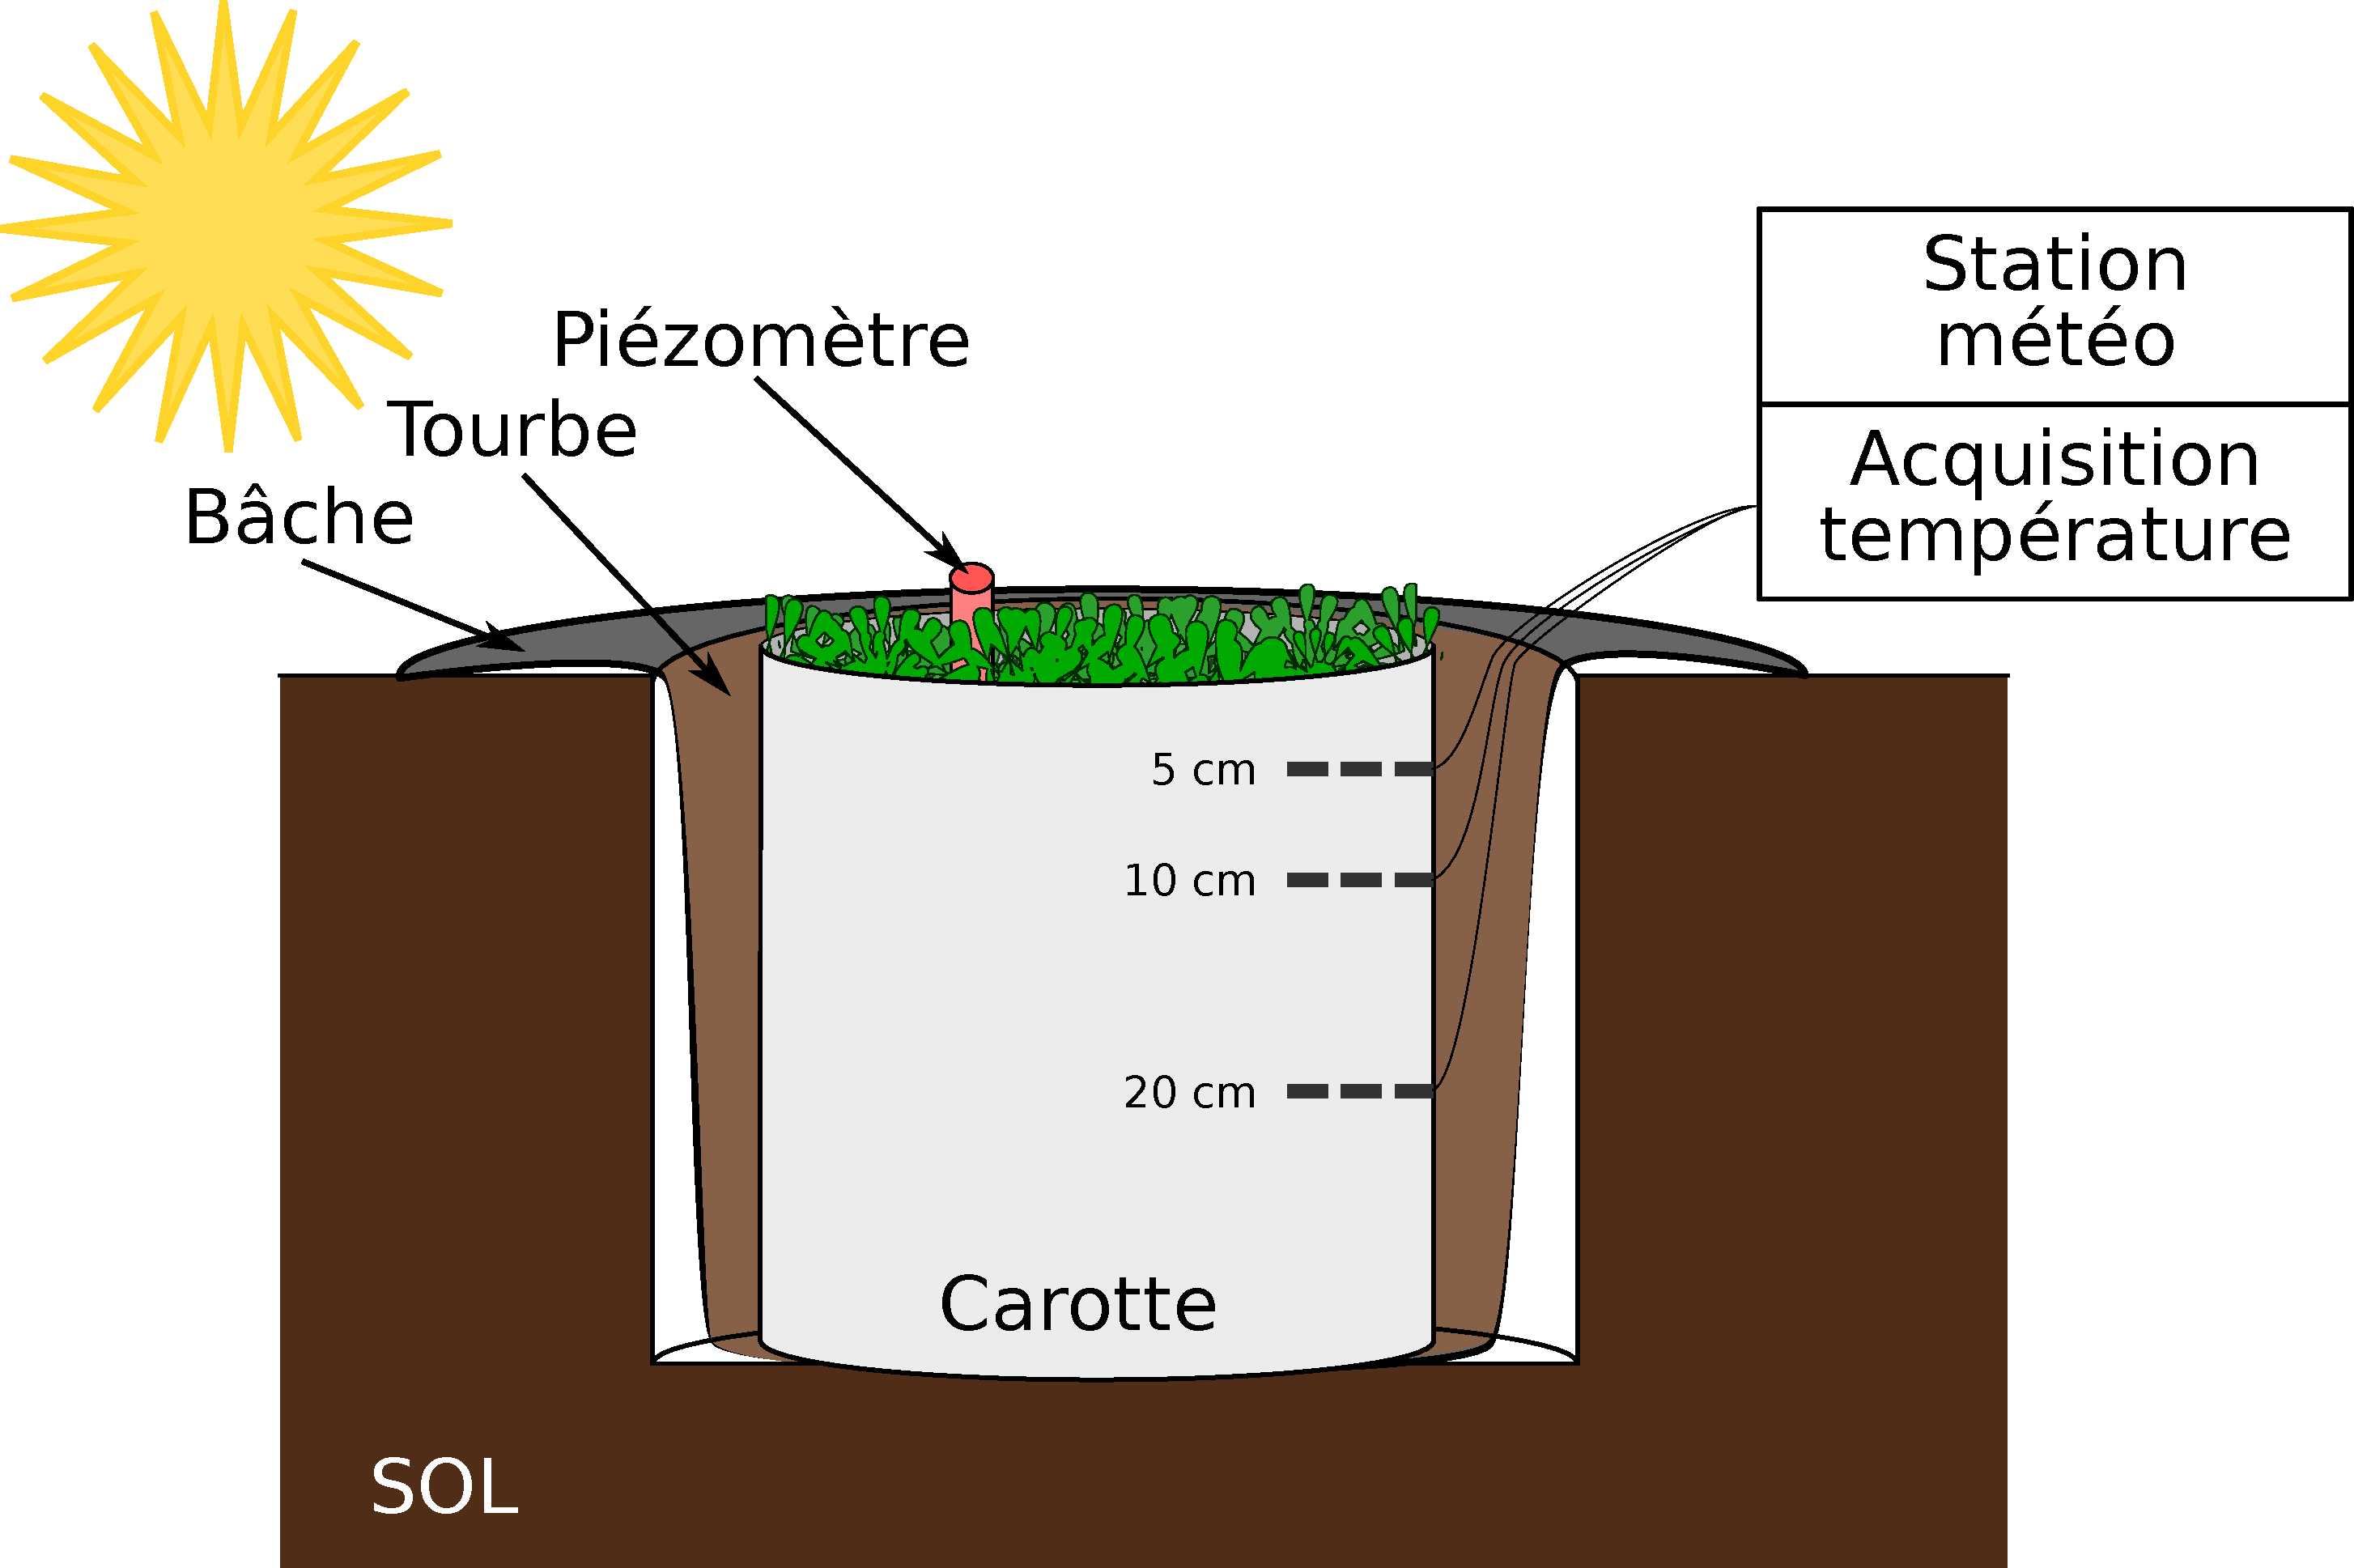
\includegraphics[width=.6\textwidth]{chap4/installation}
\caption{Schéma d'un mésocosme}
\label{fig:mesocarte}
\end{figure}

\section{Résultats}

\subsection{Expérimentation A}

\textbf{Niveau de la nappe}

Pendant la phase de dessiccation de l'expérimentation A, on observe une baisse du niveau de la nappe pour les placettes contrôles comme pour les placettes traitements (Figure~\ref{fig:HMzi}--A).
Cependant les placettes du groupe Contrôle ont un niveau de nappe relativement élevé jusqu'au 24 juin puis ce niveau baisse fortement alors que les placettes du groupe Dessiccation ont un niveau de nappe qui diminue de façon plus continue sur l'ensemble de la phase.
La remontée du niveau de la nappe s'effectue de façon similaire pour les deux groupes.
Enfin après la phase de ré-humectation, le niveau de la nappe baisse à nouveau, plus rapidement pour le groupe Dessiccation que pour le groupe Contrôle.


\begin{figure}
\centering
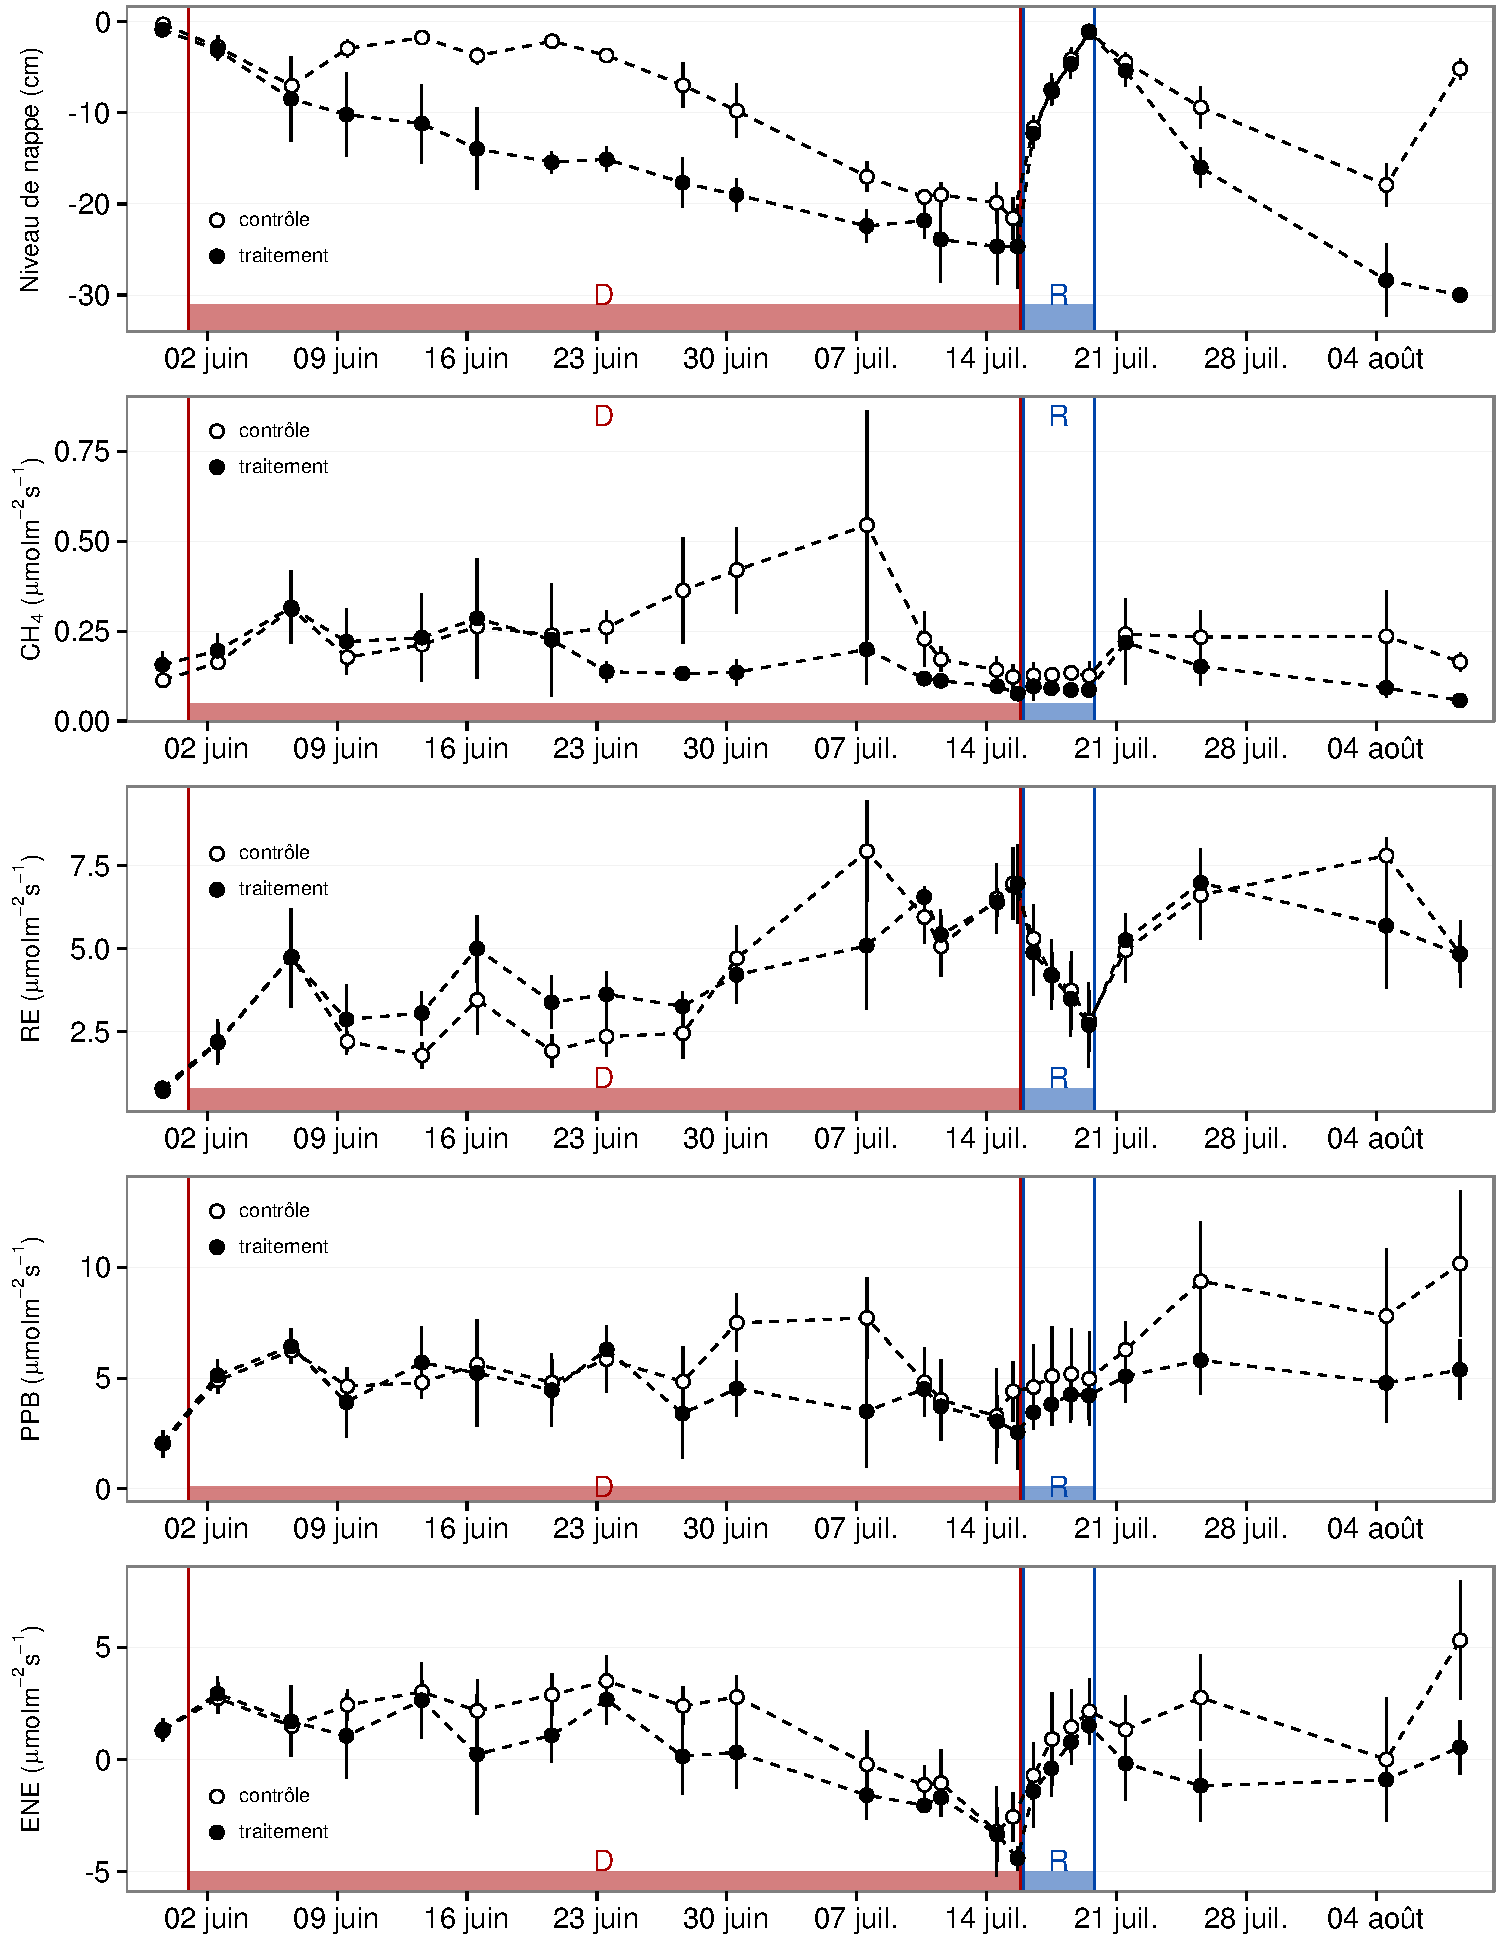
\includegraphics[width=1.15\textwidth, center]{chap4/expA_flux}
\caption{Expérimentation A : Moyenne journalière du niveau de nappe en cm (A), et des flux, \chh, RE, PPB, ENE en \si{\uml}, B, C, D, E. Les cadres et bandes colorées correspondent à la phase de dessiccation (D) en rouge et à la phase de réhumectation (R) en bleu.}
\label{fig:HMzi}
\end{figure}

\textbf{Flux de \chh}

Les émissions de \chh, varient de 0 et \SI{0.3}{\uml}.
Elles sont similaires entre les deux groupes jusqu'au 24 juin 2013, date à partir de laquelle elles divergent (Figure~\ref{fig:HMzi}--B).
À cette date les émissions du groupe contrôle augmentent rapidement pour atteindre \SI{0.55(031)}{\uml} tandis que celles du groupe traité restent stable.
À la fin de la phase de dessiccation, mi-juillet, les deux groupes retrouvent des niveaux d'émission similaires compris entre \num{0.1} et \SI{0.2}{\uml}.
Ces niveaux restent constant pendant toute la phase de réhumectation, avant d'augmenter légèrement par la suite pour se situer entre \SI{0.25}{\uml} et \SI{0.2}{\uml}.

\textbf{Flux de \coo}

Pendant la phase de dessiccation, les valeurs de la RE tendent à augmenter quel que soit le groupe de placettes considéré (Figure~\ref{fig:HMzi}--C).
Ces valeurs inférieures à \SI{2.5}{\uml} début juin, atteignent environ \SI{7}{\uml} pour les deux groupes mi-juillet, avant la réhumectation.
Cependant la RE du groupe Dessiccation augmente régulièrement pendant l'ensemble de cette phase jusqu'à \SI{3.26(046)}{\uml} , tandis que les valeurs du groupe Contrôle restent, dans un premier temps, stable jusque fin juin (\SI{2.45(075)}{\uml}).
%La RE de ce groupe vaut alors \SI{2.45(075)}{\uml} contre \SI{3.26(046)}{\uml} pour le groupe traité.
%Cet écart, pouvant varier dans le temps,  étant installé depuis le 9 juin
À partir de début juillet, les valeurs de RE du groupe Contrôle augmentent fortement dépassant les valeurs du groupe Dessiccation.
La Re de ce groupe atteint un maximum à \SI{7.93(152)}{\uml} le 8 juillet avant de retrouver des valeurs proche de celles observées dans le groupe Dessiccation.
Cette augmentation brusque correspond temporellement à celle observé, pour le même groupe, dans les flux de \chh.
Lors de la phase de réhumectation, les flux de RE diminuent de façon très similaire pour les deux groupes pour atteindre \SI{2.75}{\uml} en juin.
Ce minimum reste cependant plus élevé que les valeurs mesurées initialement.
Après la phase de réhumectation, les flux des deux groupe restent relativement proches pendant le reste des mesures, où ils remontent à mesure que le niveau de la nappe diminue à nouveau.

Pour les deux groupes, les flux de PPB restent stables pendant la phase de dessiccation (Figure~\ref{fig:HMzi}--D) :
entre 5 et \SI{6}{\uml} (\SI{5.29(076)}{\uml} de moyenne pour les deux groupes) jusqu'au 24 juin.
Ensuite comme pour le \chh et la RE, les valeurs de la PPB du groupe Contrôle augmentent et s'écartent de celles mesurées dans le groupe Dessiccation,
À la fin de cette phase de dessiccation les flux redeviennent identiques entre les traitements.
Par ailleurs, à la fin de cette phase, les flux diminuent légèrement atteignant un minimum proche de \SI{3}{\uml}.
Pendant la phase de réhumectation, la PPB augmente légèrement pour les deux groupes.
La PPB dans le groupe de contrôle a des valeurs supérieures à celles du groupe Dessiccation.
Après la réhumectation, la PPB augmente pour les deux groupes, avec un maximum de \SI{5.83(161)}{\uml} pour le groupe Dessiccation et de \SI{10.17(330)}{\uml} pour le groupe Contrôle.


L'ENE est systématiquement supérieure pour le groupe Contrôle, avec une cinétique parallèle des flux pour les deux groupes (Figure~\ref{fig:HMzi}--E).
Pendant la phase de dessiccation, l'ENE reste relativement constante jusque fin juin avec une valeur moyenne pour les deux groupes de \SI{1.18(058)}{\uml}.
L'écart entre le groupe Contrôle et le groupe Dessiccation tend à augmenter du 10 au 30 juin environ, avant que les valeurs du groupe de Contrôle ne rejoignent celles du groupe Dessiccation.
Au delà du 24 juin, l'ENE baisse fortement pour les deux groupes pour atteindre un minimum proche de \SI{-4.5}{\uml}.
Pendant la phase de réhumectation l'ENE monte rapidement pour atteindre \num{1.52(036)} et \SI{2.15(147)}{\uml} pour le groupe Contrôle et de groupe Dessiccation respectivement.
Après la réhumectation, l'ENE du groupe Contrôle varie en suivant généralement les variations du niveau de nappe.
Pour le groupe traité, l'ENE baisse par rapport au maximum atteint lors de la réhumectation puis se stabilise autour de 0.

L'effet des variations du niveau de la nappe sur la PPB est quasiment nul (Figure~\ref{fig:hm_wtl}--E), même si la PPB semble diminuer aux plus fortes profondeurs.
Les variations de la RE sont principalement liée au niveau de la nappe (Figure~\ref{fig:hm_wtl}--C) Par conséquent, les variation de RE se répercutent sur l'ENE (Figure~\ref{fig:hm_wtl}--G).
Pour le \chh il est également difficile de distinguer des tendances générales entre les flux et les niveaux de nappe (Figure~\ref{fig:hm_wtl}--A).

\begin{figure}
\centering
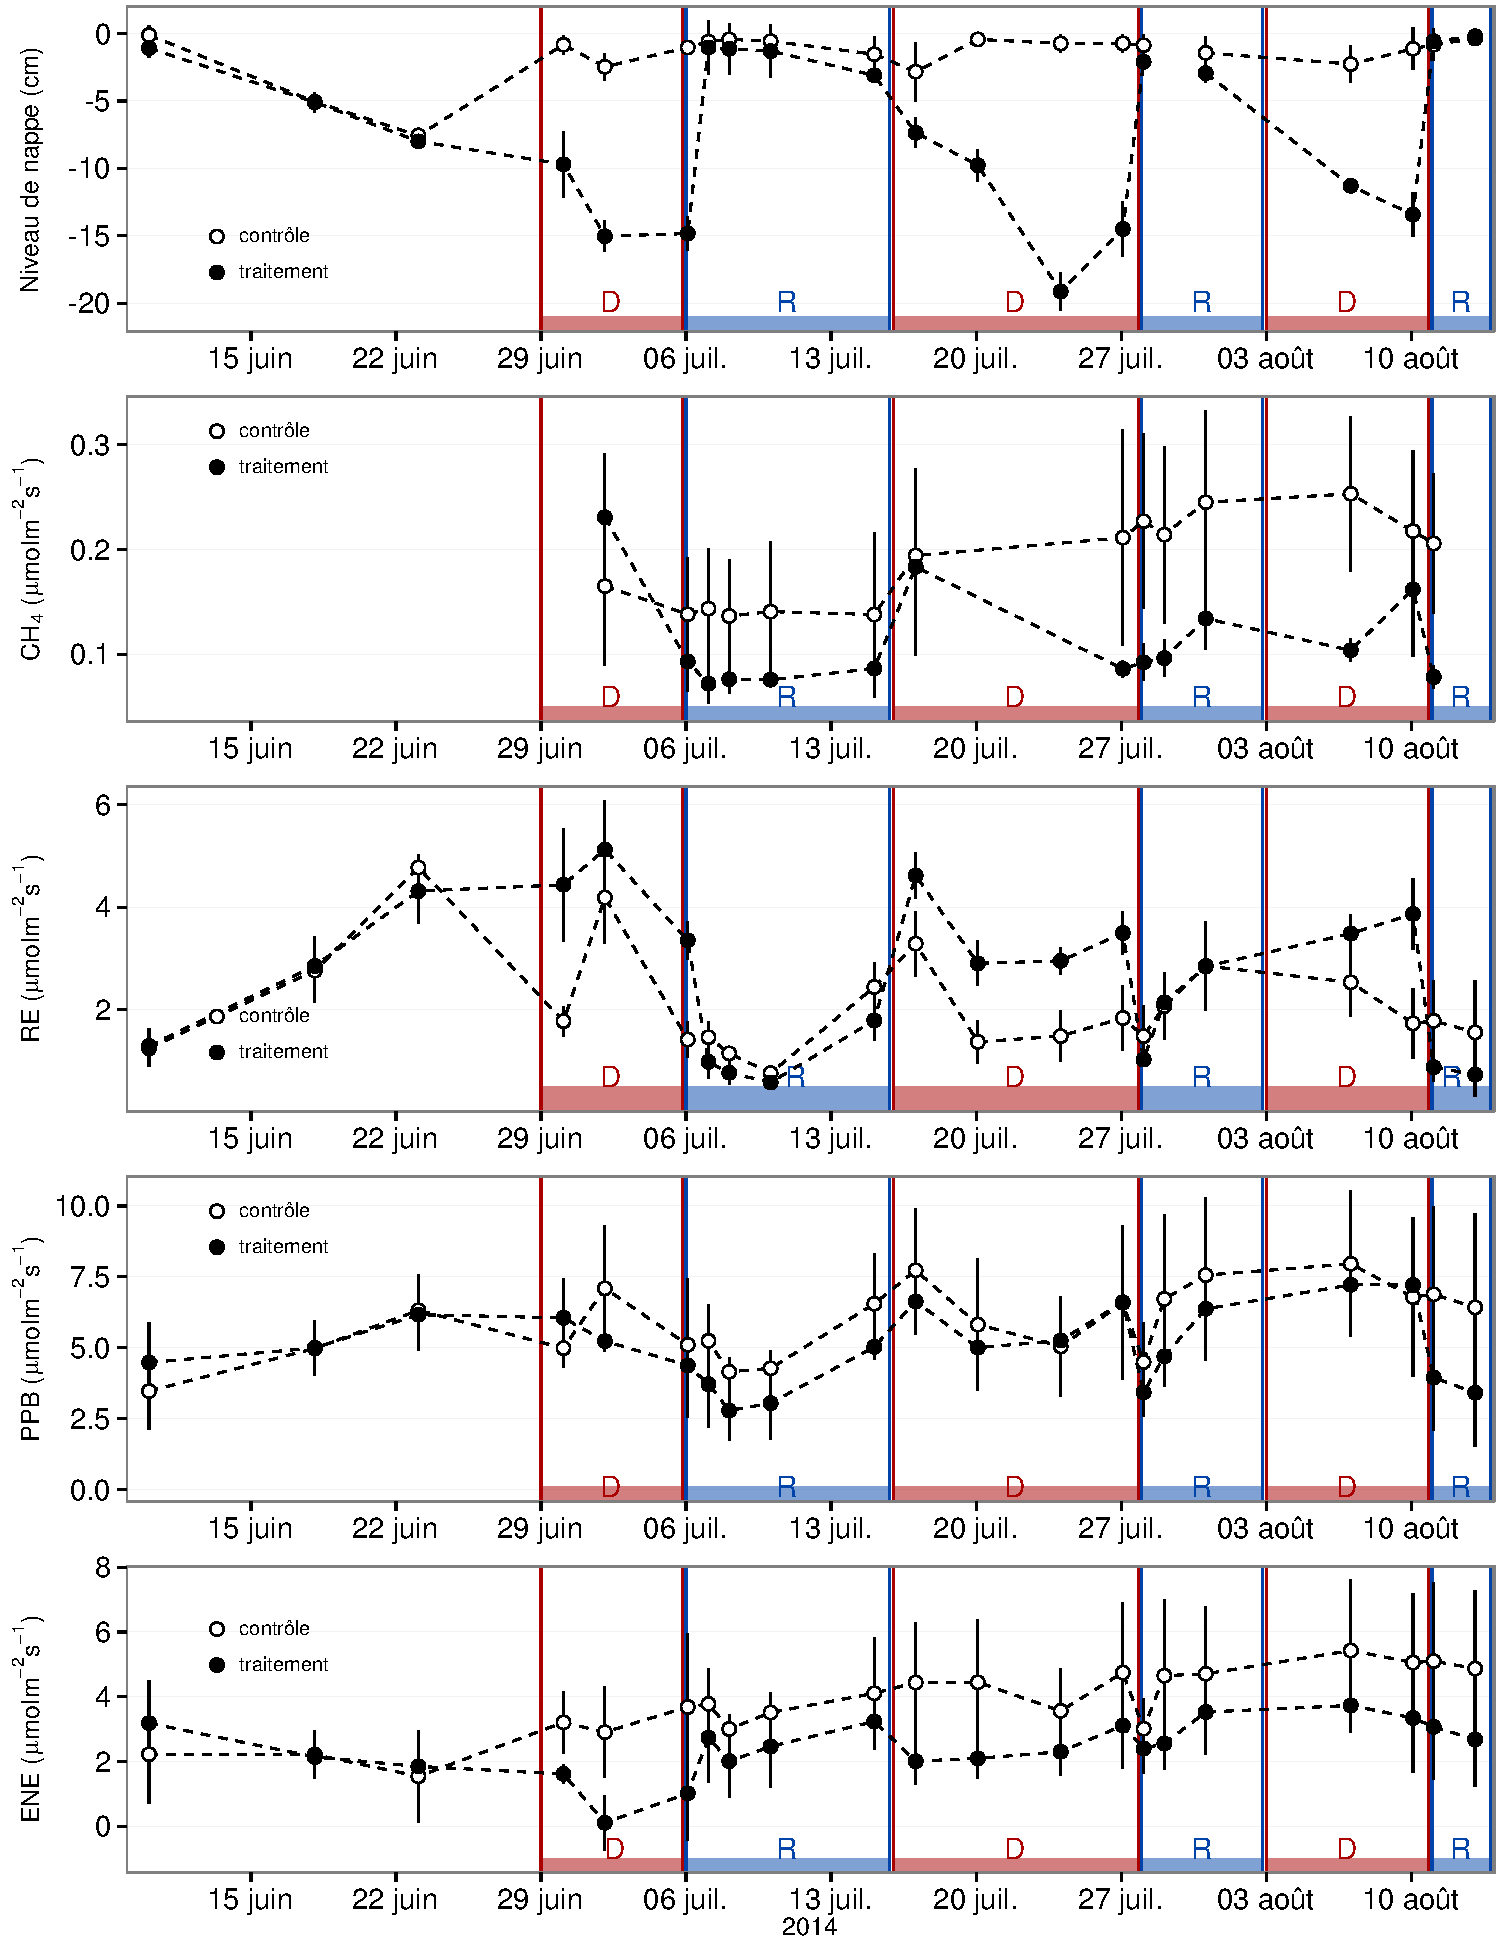
\includegraphics[width=1.15\textwidth, center]{chap4/expB_flux}
\caption{Expérimentation B : Moyenne journalière du niveau de nappe en cm (A), et des flux, \chh, RE, PPB, ENE en \si{\uml}, B, C, D, E. Les cadres et bandes colorées correspondent aux phases de dessiccation (D) en rouge et aux phases de réhumectation (R) en bleu.}
\label{fig:HMty}
\end{figure}

\subsection{Expérimentation B}

Contrairement à l'expérimentation A, le niveau de nappe du groupe Contrôle de l'expérimentation B reste relativement constant pendant l'ensemble de la période de mesure.
Le drainage artificiel du groupe Dessiccation permet d'abaisser le niveau de la nappe d'une quinzaine de centimètres en moyenne pour chaque cycle (Figure~\ref{fig:HMty}--A).

%À l'exception du point mesuré lors de la première phase de dessiccation, les valeurs du groupe de contrôle sont systématiquement supérieures à celles du groupe traité.
Les flux de \chh moyen varient entre \num{0.07} à \SI{0.34}{\uml}.
Les flux du groupe Contrôle, à l'exception de la première mesure, sont supérieurs aux flux du groupe Dessiccation, (moyennes globales de \num{0.20(006)} et \SI{0.11(005)}{\uml}, respectivement.
Les émissions du groupe Contrôle tendent à augmenter sur la période de mesure.
Une tendance similaire, est également visible pour le groupe Dessiccation.
Concernant les cycles de dessiccation/réhumectation, il est difficile de dégager des comportements communs entre eux, même si l'assèchement conduit à une baisse des émissions (Figure~\ref{fig:HMty}--B)
Cette relation, mise en exergue pas un nombre de points très faible, n’apparaît cependant pas sur l'ensemble des données (Figure~\ref{fig:hm_wtl}--B).
Un pic d'émission de \chh est également à noter pour chaque cycle pendant la phase de dessiccation.

La RE varie pour les deux groupes entre \num{0.42} et \SI{5.12}{\uml} (Figure~\ref{fig:HMty}--C)).
Avant le démarrage des manipulations du niveau de la nappe, les valeurs des deux groupes sont très proches et augmentent tandis que le niveau de nappe diminue.
Pendant les phases de dessication, les valeurs du groupe Dessiccation sont systématiquement supérieures, de \num{1.5} à \SI{1.8}{\uml}en moyenne par phase, par rapport à celle du groupe Contrôle.
À l'inverse pendant les phases de réhumectation les flux entre les deux groupes sont beaucoup plus proches avec une tendance de la RE du groupe Contrôle à être supérieure à celle du groupe Dessiccation.
La RE du groupe traité est systématiquement plus faible pendant les phases de réhumectations que pendant les phases de dessiccations.
En moyenne la RE vaut respectivement \num{2.28(100)} et \SI{3.86(080)}{\uml} pour les groupes Contrôle et Dessiccation pendant les phases de dessiccation et \num{1.70(062)} et \SI{1.51(098)}{\uml} pendant les phases de réhumectation.
%Avant le début des traitement d'assèchement, les flux de la RE sont proches pour les deux groupes tandis qu'après, leurs comportements diffèrent (Figure~\ref{fig:HMty}--C)).
%Pendant les phases de dessiccation la RE du groupe traité est supérieure à celle du groupe de contrôle.
%La relation semble s'inverser pendant les phases de réhumectation, du moins pour les cycles 1 et 3, car pendant la phase de réhumectation du cycle 2 les deux groupes ont des valeurs similaires.

Sur l'ensemble de la période de mesure la PPB est comprise entre \num{2.78} et \SI{7.96}{\uml}.
Avant le début des traitements les flux des deux groupes sont similaires (Figure~\ref{fig:HMty}--D).
À partir de la première phase de dessiccation, la PPB du groupe Contrôle supérieure à celle du groupe Dessiccation.
Pour les deux groupes, la PPB est plus importante lors des phases de dessiccation comparée aux phase de réhumectation, avec des moyennes respectives de \num{6.35(219)} contre \num{5.80(220)} pour le groupe Contrôle et de \num{5.95(146)} contre \SI{4.05(160)}{\uml} pour le groupe Dessiccation.

Les valeurs d'ENE mesurées sont comprises entre \num{0.11} et \SI{5.42}{\uml}, elles ont tendance à augmenter au cours du temps.
Passé la période pré-traitements pendant laquelle les flux de l'ENE sont similaires pour les deux groupes l'ENE du groupe Contrôle est systématiquement supérieure à celle du groupe Dessiccation (Figure~\ref{fig:HMty}--E).
%Le premier cycle de dessiccation/réhumectation divise les deux groupes : le groupe de contrôle ayant des valeurs d'ENE plus élevées que celles du groupe traité.
L'évolution des deux groupes reste cependant relativement conjointe pendant la période de mesure avec pour le groupe Dessiccation une diminution récurrente de l'ENE au début de chaque phase de dessiccation.

\begin{figure}
\centering
\begin{minipage}{.5\textwidth}
\centering
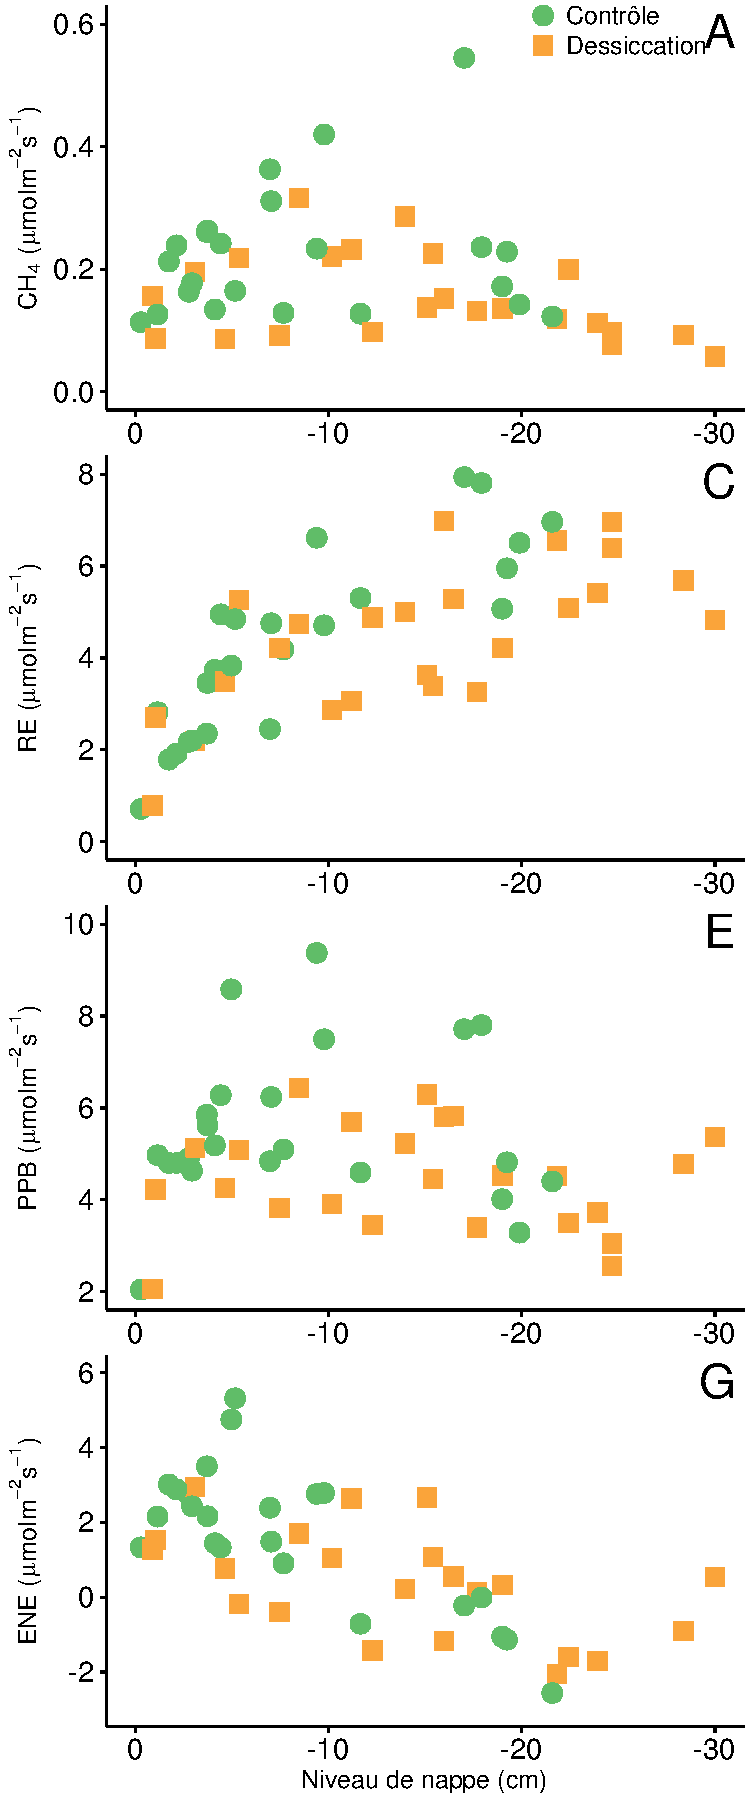
\includegraphics[width=\linewidth]{chap4/expA_fluxWTL}
\end{minipage}%
\begin{minipage}{.5\textwidth}
\centering
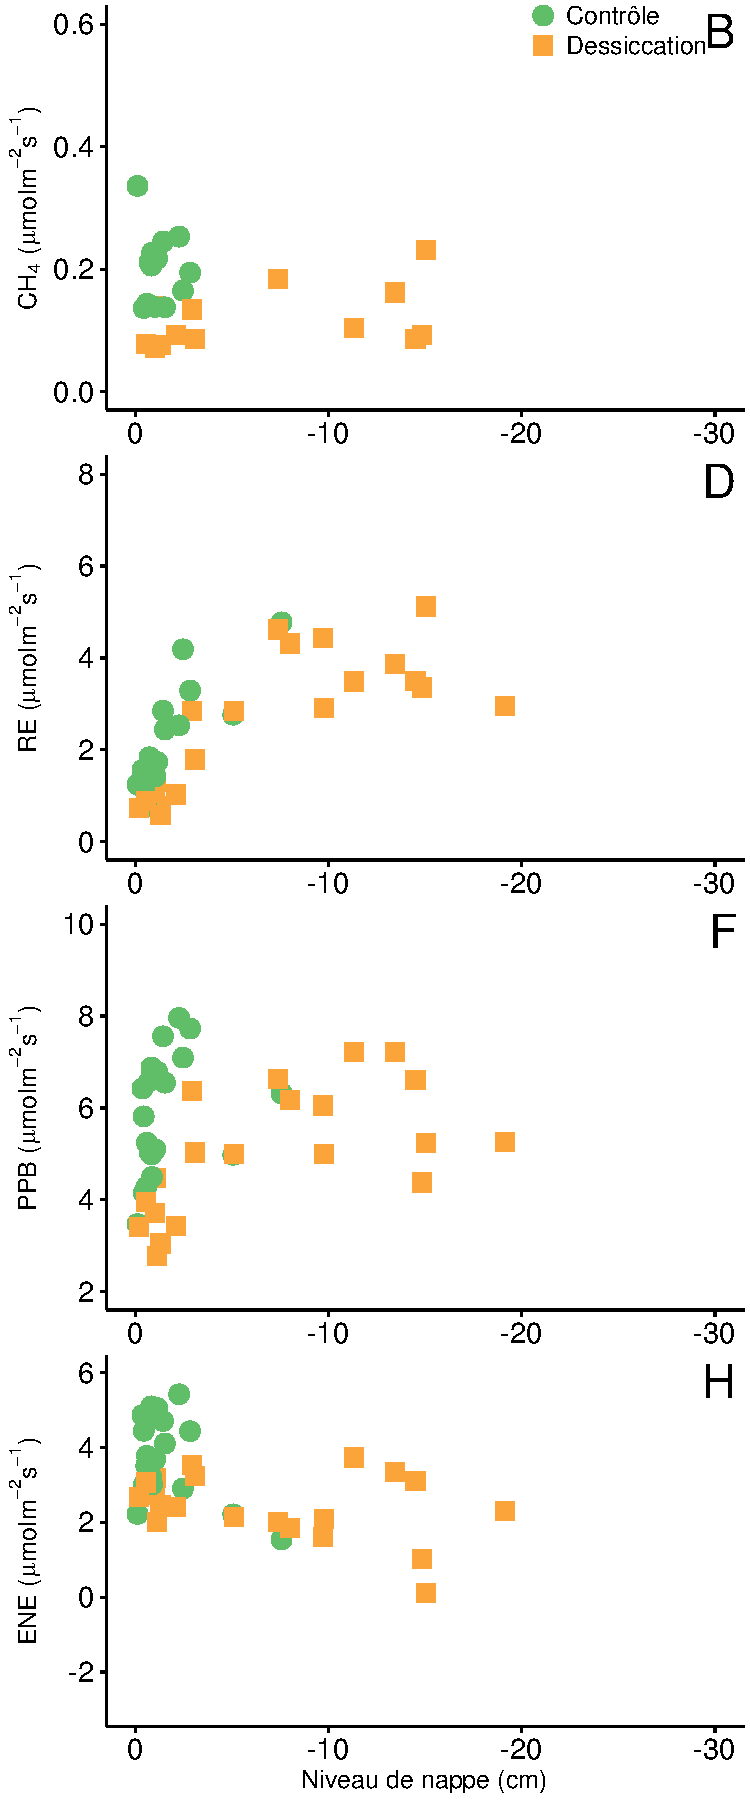
\includegraphics[width=\linewidth]{chap4/expB_fluxWTL}
\end{minipage}%
\caption{Relations entre les flux de GES et le niveau de la nappe}
\label{fig:hm_wtl}
\end{figure}

\subsection{tendances générales}

Pour les deux expérimentations une relation nette est visible entre le niveau de la nappe et l'ENE qui diminue lorsque le niveau de nappe augmente (Figure~\ref{fig:hm_wtl}--G,H).
La relation inverse est visible, pour les deux expérimentations, entre la RE et le niveau de la nappe (Figure~\ref{fig:hm_wtl}--C,D).
La PPB ne montre aucune tendance quelle que soit l'expérimentation.
On peut noter que les valeurs de PPB les plus faibles correspondent aux niveaux de nappe les plus élevés(Figure~\ref{fig:hm_wtl}--E,F).
Pour le méthane, que ce soit pour l'expérimentation A ou B, aucune tendance ne semble se dégager vis à vis du niveau de la nappe (Figure~\ref{fig:hm_wtl}--A,B).


\section{Discussion}

\subsection{Comparaison aux mesures \textit{in-situ}}
%CH4

Les flux moyen de \chh mesurés dans les mésocosmes des deux expérimentations font partie des valeurs hautes mesurées sur le terrain.
Certaines campagnes dépassent nettement, en faisant plus que doubler, le maximum de \SI{0.2}{\uml} mesuré en 2014 sur la tourbière de La Guette.

Pour le \coo les flux sont généralement dans la gamme des valeurs mesurées sur la tourbière de La Guette.
Pour l'expérimentation A, l'ENE moyen est plus faible que celui mesuré sur le terrain la même année : \num{0.81} contre \SI{2.85}{\uml}.
Pour l'expérimentation B en revanche l'ENE moyen vaut \SI{0.71}{\uml} ce qui est relativement proche de celui mesuré sur le terrain : \SI{2.93}{\uml}.
Les flux de RE et de PPB sont moins fort que les flux mesurés sur le terrain mais restent dans leur gamme de valeurs.
Ces comparaisons sont par ailleurs à relativiser puisque les mesures de flux n'ont pas nécessairement lieu aux mêmes moment de la journée.


%À l'exception de la forte hausse, fin juin, début juillet, du groupe contrôle, les valeurs de méthane sont comprise entre 0 et \SI{0.3}{\uml}.
%Ces valeurs sont un peu plus élevée, mais du même ordre de grandeur que celles mesurées sur le terrain.
%
%Les émissions de \chh mesuré lors de l'expérimentation B sont du même ordre de grandeur, entre 0 et \SI{0.3}{\uml}, que celles mesurées \textit{in-situ}, sur la tourbière de La Guette.
%
%% RE
%Les valeurs de RE mesurées sont dans la gamme de celles mesurées sur le terrain, avec cependant des maximums moins importants.
%
%Les valeurs RE mesurées sur les mésocomes sont plus faible que celle relevées directement sur la tourbière de La Guette avec un maximum moyen à 5 contre \SI{8}{\uml} mesuré sur le site.

% PPB

Comme pour la RE, les flux de PPB sont du même ordre de grandeur que ceux mesurés sur le terrain, mais dans la gamme basse : les maximas moyens mesurés dans les mésocosmes sont d'environ \num{7.5} pour des valeurs de \SI{13}{\uml} mesuré directement sur la tourbière.

\subsection{Effet des variations du niveau de la nappe sur les flux de gaz}

Les résultats de ces deux expérimentations montrent une augmentation de la RE quand le niveau de la nappe diminue.
Ceci est en accord avec les résultats d'autres études que ce soit in-situ \citep{ballantyne2014} ou en mésocosmes \citep{blodau2004,dinsmore2009}.
Dans ces deux dernières publications, la baisse du niveau de la nappe diminue la PPB.
Pas de variations significatives de la PPB avec le niveau de la nappe n'est visible dans les données présentées, même si une légère tendance semble émergée aux plus fortes profondeur de nappe pour l'expérimentation A.
Cette absence d'effet du niveau de la nappe sur la PPB peut, être liée à la profondeur des mésocosmes (\SI{30}{\centi\metre}).
En effet dans \citet{blodau2004} et \citet{dinsmore2009}, les mésocosmes utilisés sont plus grands, 75 et \SI{41}{\centi\metre} respectivement, ont permis d'abaisser le niveau de l'eau au delà de \SI{-30}{\centi\metre}.
Cette limite a été rapportée plusieurs fois comme étant un seuil au delà duquel son observés des changements importants \citep{blodau2004,peichl2014}.
Ce seuil est expliqué comme étant la limite au delà de laquelle les forces de capillarités ne permettent plus d'alimenter en eau les sphaignes \citep{rydin2013a,ketcheson2014}.
Il résulte des constats précédents qu'une baisse du niveau de nappe, faisant augmenter la RE et ne changeant pas ou peu la PPB, conduit à une baisse de l'ENE.
Cette diminution de l'ENE est cohérente avec la littérature, que ce soit des expérimentations en mésocosmes \citep{aerts1997,blodau2004}, ou in-situ \citep{bubier2003,sonnentag2010}.
Malgré tout l'extrapolation de ses résultats à d'autres situations n'est pas aisée car fortement fonction du contexte.
D'autre études n'ont, par exemple, pas observé d'influence du niveau de la nappe sur la RE \citep{updegraff2001}.
Par ailleurs \citet{laiho2006} a montré l'importance du contexte et notamment celui de l'échelle de temps considéré qui peut impliquer des phénomènes différents et donc avoir des conséquences différentes.

La dépendance entre les flux de \chh et le niveau de la nappe, devant conduire à une baisse des émissions quand le niveau de la nappe diminue, comme décrite dans \citet{aerts1997}, \citet{pelletier2007} ou \citet{turetsky2008}, n'a pas été clairement observée.
Ce constat rejoins d'autres études dans lesquelles une relation inverse ou un absence de relation a été trouvé entre le \chh et le niveau de la nappe \citet{kettunen1996,bellisario1999,treat2007}.
L'observation d'un pic de méthane suivant de quelques jours une phase de hausse du niveau de la nappe, est également rapportée par \citet{kettunen1996}. \textbf{(And so what ?)}


%\subsection{Dessication}
%
%Lors des phases de dessiccations, les deux expérimentations montrent une hausse de la RE, que l'assèchement soit sur une période longue (expérimentation A) ou plus courte (expérimentation B).
%À cause des conditions météorologiques présentes lors de l'expérimentation A, le groupe de contrôle subit également un assèchement et donc une hausse de sa RE.
%À l'inverse les conditions météorologique moins ensoleillée de l'expérimentation B ont permis d'observer une différence nette entre d'assèchement du groupe traité et celui du groupe de contrôle.
%Pour cette expérimentation, la différence entre la RE des deux groupes est statistiquement différente (p<0.05) pendant les phases de dessiccation mais non pendant les phases de réhumectation.
%À l'exception du cycle 3 pour lequel la différence entre traitement et contrôle est également significative.
%La RE est donc impactée de façon significative lors d'un assèchement et même si les différences ne sont significative que pour R3, il est intéressant de noter que pendant les phases de réhumectation la RE du groupe traité tend à être plus faible que celle du groupe de contrôle.
%Ainsi les cycles de dessiccation/réhumectation semblent augmenter les extrêmes de la gamme de valeur de la RE.
%
%La baisse du \chh observé dans l'expérimentation A, 
%
%
%Discuter les hausses de CH4 et de RE à partir du 23 juin pour Zi.
%
%\subsection{Réhumectation}
%
%La réhumectation après une phase de dessication fait baisser la RE, que ce soit pour l'expérimentation A ou l'expérimentation B.
%
%Il semble y avoir une émission de \chh suite aux phases de réhumectation, mais avec un certain temps de latence.
%L'expérimentation A le montre  de façon relativement clair.
%Par contre si des pics sont également visible dans l'expérimentation B, la faible durée des cycles ne permet pas de déterminer s'ils sont liés à la réhumectation ou à la phase de dessication qui suit.

\subsection{Effet cycles multiples}
